\documentclass[letter, 10pts]{article}
\usepackage[monocolor]{../math232/ahsansabit}
\usepackage[]{float}
\usepackage{tikz}
\usepackage{tikz-3dplot}
\usepackage[outline]{contour} % glow around text
\usepackage{xcolor}
\usepackage{pdfpages}
\usepackage{physics}
\usepackage{multicol}
\title{Quantum Mechanics : : Homework 11}
\author{Ahmed Saad Sabit, Rice University}
\date{\today}
\newcommand{\hb}{\hbar}
\newcommand{\U}{\uparrow}
\newcommand{\D}{\downarrow}
\usepackage[]{braket}
\begin{document}
\maketitle



\section*{Problem 01} 
General matrix representation of an operator $X$ if basis vectors are given by 
$\{ \ket{1}, \ket{2}, \ket{3}, \ket{4}, \ket{5} \}$ is (\emph{Sakurai eq 1.73})
\[
\begin{bmatrix}
\langle 1 \mid X \mid 1 \rangle & \langle 1 \mid X \mid 2 \rangle & \langle 1 \mid X \mid 3 \rangle & \langle 1 \mid X \mid 4 \rangle & \langle 1 \mid X \mid 5 \rangle \\
\langle 2 \mid X \mid 1 \rangle & \langle 2 \mid X \mid 2 \rangle & \langle 2 \mid X \mid 3 \rangle & \langle 2 \mid X \mid 4 \rangle & \langle 2 \mid X \mid 5 \rangle \\
\langle 3 \mid X \mid 1 \rangle & \langle 3 \mid X \mid 2 \rangle & \langle 3 \mid X \mid 3 \rangle & \langle 3 \mid X \mid 4 \rangle & \langle 3 \mid X \mid 5 \rangle \\
\langle 4 \mid X \mid 1 \rangle & \langle 4 \mid X \mid 2 \rangle & \langle 4 \mid X \mid 3 \rangle & \langle 4 \mid X \mid 4 \rangle & \langle 4 \mid X \mid 5 \rangle \\
\langle 5 \mid X \mid 1 \rangle & \langle 5 \mid X \mid 2 \rangle & \langle 5 \mid X \mid 3 \rangle & \langle 5 \mid X \mid 4 \rangle & \langle 5 \mid X \mid 5 \rangle
\end{bmatrix}
\]





\subsection*{(a)} 
The basis we are going to use, 
\[
\{
	\ket{2,2}, 
	\ket{2,1}, 
	\ket{2,0},
	\ket{2,-1},
\ket{2,-2} \}
\] 
The first matrix is for 
\[
\hat{\vec{J}}^2 \ket{j,m} = \hb^2 j (j+1) \ket{j,m}
\] 

\begin{align*}
\hat{J}^2 \ket{2,2} &= \hbar^2 6 \ket{2,2}, \\
\hat{J}^2 \ket{2,1} &= \hbar^2 6 \ket{2,1}, \\
\hat{J}^2 \ket{2,0} &= \hbar^2 6 \ket{2,0}, \\
\hat{J}^2 \ket{2,-1} &= \hbar^2 6 \ket{2,-1}, \\
\hat{J}^2 \ket{2,-2} &= \hbar^2 6 \ket{2,-2}
\\ \implies
\hat{J}^2 &=		     
\hb^2 
\begin{bmatrix}
6 & 0 & 0 & 0 & 0 \\
0 & 6 & 0 & 0 & 0 \\
0 & 0 & 6 & 0 & 0 \\
0 & 0 & 0 & 6 & 0 \\
0 & 0 & 0 & 0 & 6
\end{bmatrix}
\end{align*}

The second matrix is for 
\[
\hat{J}_z \ket{j,m} = \hb m \ket{j,m}
\] 

\begin{align*}
	\hat{J}_z \ket{2,2} &= 2\hbar \ket{2,2}, \\
\hat{J}_z \ket{2,1} &= \hbar \ket{2,1}, \\
\hat{J}_z \ket{2,0} &= 0, \\
\hat{J}_z \ket{2,-1} &= -\hbar \ket{2,-1}, \\
\hat{J}_z \ket{2,-2} &= -2\hbar \ket{2,-2} \\ \implies 
\hat{J}_z &= 
\hb 
\begin{bmatrix}
2 & 0 & 0 & 0 & 0 \\
0 & 1 & 0 & 0 & 0 \\
0 & 0 & 0 & 0 & 0 \\
0 & 0 & 0 & -1 & 0 \\
0 & 0 & 0 & 0 & -2
\end{bmatrix} 
\end{align*}

The third matrix is the $(+)$ ladder matrix 
\[
\hat{J}_\pm \ket{j,m} = \hb 
\sqrt{j (j+1) - m (m\pm 1) } 
\ket{j, m \pm 1}
\] 

\begin{align*}
\hat{J}_+ \ket{2,2} &= 0, \\
\hat{J}_+ \ket{2,1} &= \hbar \sqrt{4} \ket{2,2}, \\
\hat{J}_+ \ket{2,0} &= \hbar \sqrt{6} \ket{2,1}, \\
\hat{J}_+ \ket{2,-1} &= \hbar \sqrt{6} \ket{2,0}, \\
\hat{J}_+ \ket{2,-2} &= \hbar \sqrt{4} \ket{2,-1}, \\
\implies \hat{J}_+ &=  \hb
\begin{bmatrix}
0 &  \sqrt{4} & 0 & 0 & 0 \\
0 & 0 & \sqrt{6} & 0 & 0 \\
0 & 0 & 0 & \sqrt{6} & 0 \\
0 & 0 & 0 & 0 & \sqrt{4} \\
0 & 0 & 0 & 0 & 0
\end{bmatrix}
\end{align*}

The other third matrix for the $(-)$ ladder matrix 
\begin{align*}
\hat{J}_- \ket{2,2} &= \hbar \sqrt{4} \ket{2,1}, \\
\hat{J}_- \ket{2,1} &= \hbar \sqrt{6} \ket{2,0}, \\
\hat{J}_- \ket{2,0} &= \hbar \sqrt{6} \ket{2,-1}, \\
\hat{J}_- \ket{2,-1} &= \hbar \sqrt{4} \ket{2,-2}, \\
\hat{J}_- \ket{2,-2} &= 0. \\ 
\implies \hat{J}_- &= 
\hbar
\begin{bmatrix}
0 & 0 & 0 & 0 & 0 \\
\sqrt{4} & 0 & 0 & 0 & 0 \\
0 & \sqrt{6} & 0 & 0 & 0 \\
0 & 0 & \sqrt{6} & 0 & 0 \\
0 & 0 & 0 & \sqrt{4} & 0
\end{bmatrix}
\end{align*}





\subsection*{(b)} 
I will include the $\hb^2$ factor at the end, for now consider $\hb = 1$. 
\begin{align*}
	[J_z , J_+] &= J_z J_+ - J_+ J_z  \\ 
	&= 
\begin{bmatrix}
2 & 0 & 0 & 0 & 0 \\
0 & 1 & 0 & 0 & 0 \\
0 & 0 & 0 & 0 & 0 \\
0 & 0 & 0 & -1 & 0 \\
0 & 0 & 0 & 0 & -2
\end{bmatrix} 
\begin{bmatrix}
0 &  \sqrt{4} & 0 & 0 & 0 \\
0 & 0 & \sqrt{6} & 0 & 0 \\
0 & 0 & 0 & \sqrt{6} & 0 \\
0 & 0 & 0 & 0 & \sqrt{4} \\
0 & 0 & 0 & 0 & 0
\end{bmatrix} 
- 
\begin{bmatrix}
0 &  \sqrt{4} & 0 & 0 & 0 \\
0 & 0 & \sqrt{6} & 0 & 0 \\
0 & 0 & 0 & \sqrt{6} & 0 \\
0 & 0 & 0 & 0 & \sqrt{4} \\
0 & 0 & 0 & 0 & 0
\end{bmatrix} 
\begin{bmatrix}
2 & 0 & 0 & 0 & 0 \\
0 & 1 & 0 & 0 & 0 \\
0 & 0 & 0 & 0 & 0 \\
0 & 0 & 0 & -1 & 0 \\
0 & 0 & 0 & 0 & -2
\end{bmatrix} 
\end{align*}
\begin{figure}[H]
	\centering
	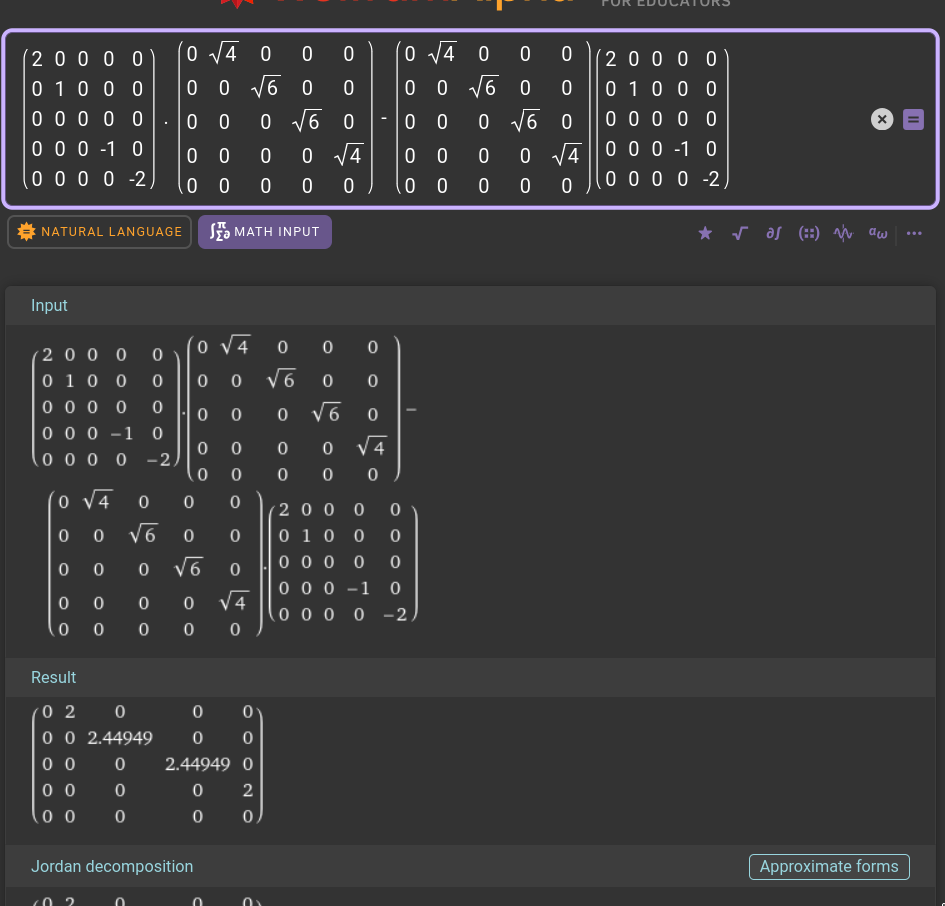
\includegraphics[width=0.8\textwidth]{./ss/11/1.png}
	\caption{./ss/11/1.png}
	\label{fig:-ss-11-1-png}
\end{figure}
\[
= \begin{bmatrix}
0 &  \sqrt{4} & 0 & 0 & 0 \\
0 & 0 & \sqrt{6} & 0 & 0 \\
0 & 0 & 0 & \sqrt{6} & 0 \\
0 & 0 & 0 & 0 & \sqrt{4} \\
0 & 0 & 0 & 0 & 0
\end{bmatrix} 
\implies \hb ^2 \begin{bmatrix}
0 &  \sqrt{4} & 0 & 0 & 0 \\
0 & 0 & \sqrt{6} & 0 & 0 \\
0 & 0 & 0 & \sqrt{6} & 0 \\
0 & 0 & 0 & 0 & \sqrt{4} \\
0 & 0 & 0 & 0 & 0
\end{bmatrix}  = \hb J_+
\] 
\[
\implies 
[J_z , J_+] = \hb J_+
\] 





\newpage 
\begin{align*}
	[J_z, J_-] &= 
J_z J_- - J_- J_z 
	\\
		   &= 
		   \begin{bmatrix}
2 & 0 & 0 & 0 & 0 \\
0 & 1 & 0 & 0 & 0 \\
0 & 0 & 0 & 0 & 0 \\
0 & 0 & 0 & -1 & 0 \\
0 & 0 & 0 & 0 & -2
\end{bmatrix} 
\begin{bmatrix}
0 & 0 & 0 & 0 & 0 \\
\sqrt{4} & 0 & 0 & 0 & 0 \\
0 & \sqrt{6} & 0 & 0 & 0 \\
0 & 0 & \sqrt{6} & 0 & 0 \\
0 & 0 & 0 & \sqrt{4} & 0
\end{bmatrix}
-
\begin{bmatrix}
0 & 0 & 0 & 0 & 0 \\
\sqrt{4} & 0 & 0 & 0 & 0 \\
0 & \sqrt{6} & 0 & 0 & 0 \\
0 & 0 & \sqrt{6} & 0 & 0 \\
0 & 0 & 0 & \sqrt{4} & 0
\end{bmatrix}
		   \begin{bmatrix}
2 & 0 & 0 & 0 & 0 \\
0 & 1 & 0 & 0 & 0 \\
0 & 0 & 0 & 0 & 0 \\
0 & 0 & 0 & -1 & 0 \\
0 & 0 & 0 & 0 & -2
\end{bmatrix} 
\end{align*}
\begin{figure}[H]
	\centering
	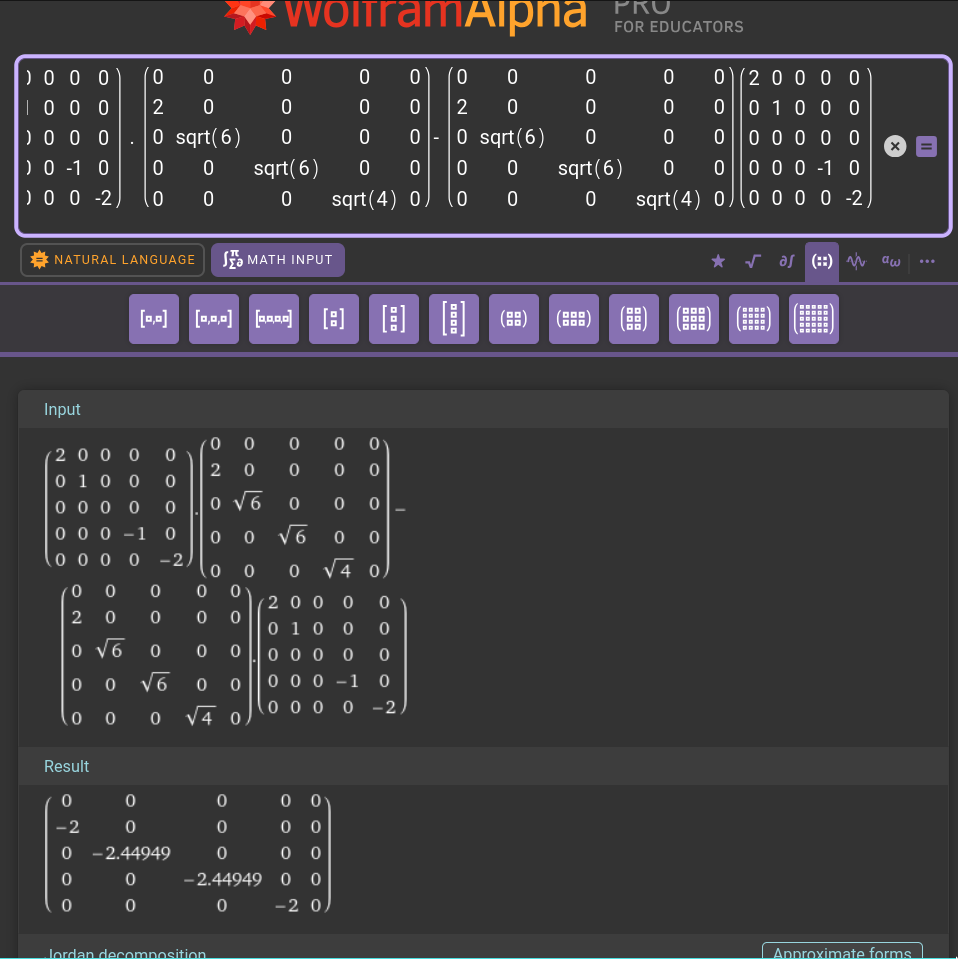
\includegraphics[width=0.8\textwidth]{./ss/11/2.png}
	\caption{}
	\label{fig:}
\end{figure}
\[
=
-
\begin{bmatrix}
0 & 0 & 0 & 0 & 0 \\
\sqrt{4} & 0 & 0 & 0 & 0 \\
0 & \sqrt{6} & 0 & 0 & 0 \\
0 & 0 & \sqrt{6} & 0 & 0 \\
0 & 0 & 0 & \sqrt{4} & 0
\end{bmatrix}
\implies -\hb^2 
\begin{bmatrix}
0 & 0 & 0 & 0 & 0 \\
\sqrt{4} & 0 & 0 & 0 & 0 \\
0 & \sqrt{6} & 0 & 0 & 0 \\
0 & 0 & \sqrt{6} & 0 & 0 \\
0 & 0 & 0 & \sqrt{4} & 0
\end{bmatrix} = - \hb J_-
\] 

\[\implies
	[J_z , J_-] = - \hb J_-
\] 



\begin{align*}
	[J_+, J_-] &= J_+ J_- - J_- J_+  \\ 
	&= 
\begin{bmatrix}
0 &  \sqrt{4} & 0 & 0 & 0 \\
0 & 0 & \sqrt{6} & 0 & 0 \\
0 & 0 & 0 & \sqrt{6} & 0 \\
0 & 0 & 0 & 0 & \sqrt{4} \\
0 & 0 & 0 & 0 & 0
\end{bmatrix}  
\begin{bmatrix}
0 & 0 & 0 & 0 & 0 \\
\sqrt{4} & 0 & 0 & 0 & 0 \\
0 & \sqrt{6} & 0 & 0 & 0 \\
0 & 0 & \sqrt{6} & 0 & 0 \\
0 & 0 & 0 & \sqrt{4} & 0
\end{bmatrix} 
- 
\begin{bmatrix}
0 & 0 & 0 & 0 & 0 \\
\sqrt{4} & 0 & 0 & 0 & 0 \\
0 & \sqrt{6} & 0 & 0 & 0 \\
0 & 0 & \sqrt{6} & 0 & 0 \\
0 & 0 & 0 & \sqrt{4} & 0
\end{bmatrix} 
\begin{bmatrix}
0 &  \sqrt{4} & 0 & 0 & 0 \\
0 & 0 & \sqrt{6} & 0 & 0 \\
0 & 0 & 0 & \sqrt{6} & 0 \\
0 & 0 & 0 & 0 & \sqrt{4} \\
0 & 0 & 0 & 0 & 0
\end{bmatrix}  
\end{align*}
\begin{figure}[H]
	\centering
	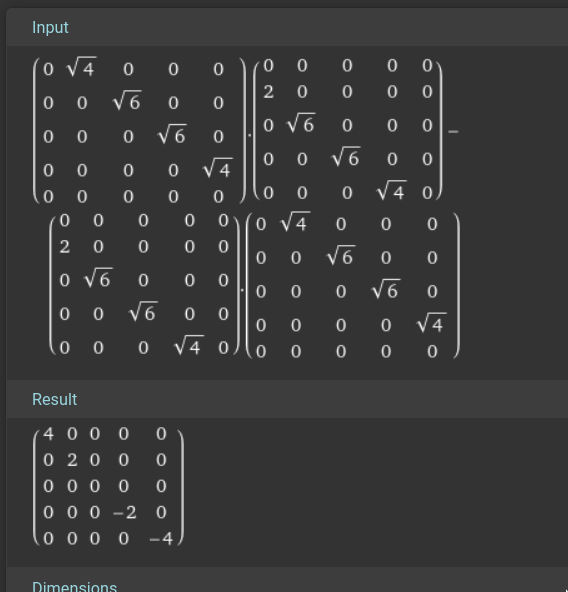
\includegraphics[width=0.8\textwidth]{./ss/11/3.png}
	\caption{./ss/11/3.png}
	\label{fig:-ss-11-3-png}
\end{figure}	
\[
= 2 
\begin{bmatrix} 2&0&0&0&0\\
0&1&0&0&0\\
0&0&0&0&0\\
0&0&0&-1&0\\
0&0&0&0&-2\end{bmatrix}  
\implies \hb^2
\begin{bmatrix} 2&0&0&0&0\\
0&1&0&0&0\\
0&0&0&0&0\\
0&0&0&-1&0\\
0&0&0&0&-2\end{bmatrix}   = 2 \hb J_z
\] 

\[
	[J_+,J_-] = 2 \hb J_z
\] 

\newpage 
We will compute 
\begin{align*}
	\frac{1}{2}(
	J_+ J_- + J_- J_+ ) + J_z^2
\end{align*}
using matrix. 
\begin{figure}[H]
	\centering
	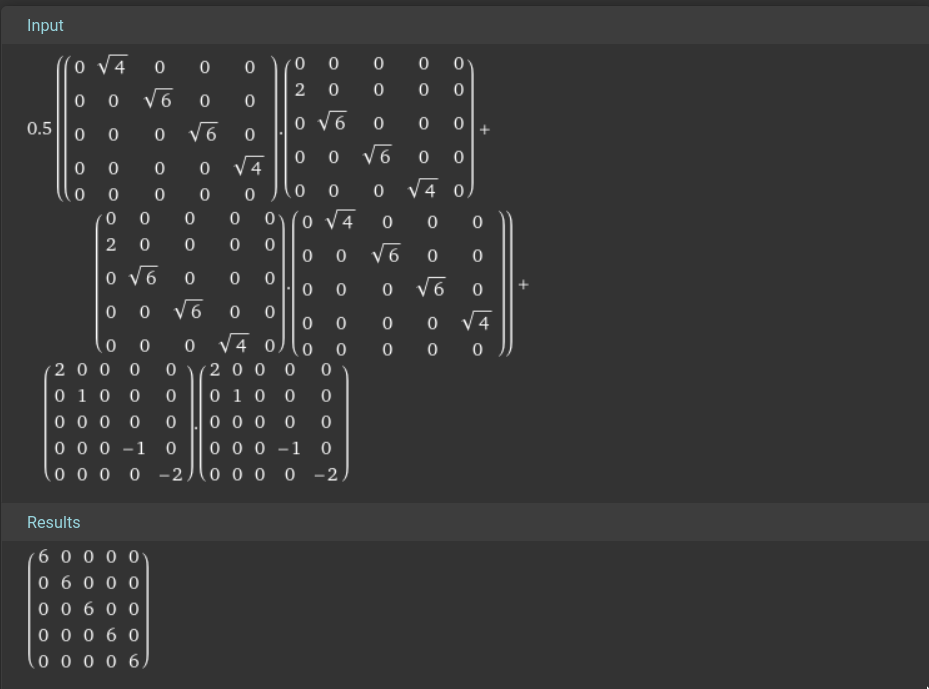
\includegraphics[width=0.8\textwidth]{./ss/11/4.png}
	\caption{./ss/11/4.png}
	\label{fig:-ss-11-4-png}
\end{figure}
\[
\begin{bmatrix} 
6 & 0 & 0 & 0 & 0 \\
0 & 6 & 0 & 0 & 0 \\
0 & 0 & 6 & 0 & 0 \\
0 & 0 & 0 & 6 & 0 \\
0 & 0 & 0 & 0 & 6
\end{bmatrix}  \implies  \hb^2
\begin{bmatrix}
6 & 0 & 0 & 0 & 0 \\
0 & 6 & 0 & 0 & 0 \\
0 & 0 & 6 & 0 & 0 \\
0 & 0 & 0 & 6 & 0 \\
0 & 0 & 0 & 0 & 6
\end{bmatrix} = 6\hb^2  \hat{I} = \vec{J}^2
\] 




\newpage
\section*{Problem 02} 
\begin{align*}
J_+ &= J_x + i J_y  \\
J_- &= J_x - i J_y \\ 
J_+ + J_- &= 2 J_x \\
\implies J_x &= \frac{1}{2} \left(J_+ + J_-\right) \\
\implies J_x^2 &= \frac{1}{4} \left(J_+ + J_-\right) \left(J_+ + J_-\right)  
= \frac{1}{4} \left(
J_+^{2} + J_+ J_- + J_- J+ + J_-^2
\right) 
= \frac{1}{4} \left(
J_+^{2} + J_+ J_- + J_- J_+ + J_-^2
\right)  \\ 
\
\\
\text{now, } 
J_x \ket{j,m} &= \frac{1}{2} J_+ \ket{j,m} + \frac{1}{2} J_- \ket{j,m} 
=
C_1 \ket{j, m+1} + C_2 \ket{j, m-1} \\ \implies
\braket{j,m | J_x | j,m } &= 0 \\
J_x^2 \ket{j,m} &= \frac{1}{4} (D_1 \ket{j, m+2} + D_2 \ket{j, m-2})
+ \frac{1}{4}
\left(
\hb^2 
\sqrt{j(j+1) - (m-1)m} 
\sqrt{j(j+1) - m(m-1)} 
\right) \ket{j, m} 
\\ 
+& 
\frac{1}{4} 
\left(
\hb ^2 
\sqrt{j(j+1) - (m+1)m} 
\sqrt{j(j+1) - (m+1)m} 
\right) \ket{j,m}
\\\implies
\braket{j,m | J_x^2  | j,m} 
&=  \frac{1}{4} 
\left(
\hb^2 j(j+1) - \hb ^2 m(m-1)  
+ \hb^2 j(j+1) - \hb ^2 m (m+1)
\right)\\
&=  \frac{\hb^2}{4} 
\left(
 j(j+1) -  m(m-1)  
+ j(j+1) - m (m+1)
\right)\\
&=  \frac{\hb^2}{4} 
\left(
 j(j+1) -  m^2 + m 
+ j(j+1) - m^2 - m 
\right)\\
&=  \frac{\hb^2}{2} 
\left(
 j(j+1) -  m^2  
\right)\\
&=  \frac{\hb^2}{2} 
\left(
 j + j^2 -  m^2  
\right)\\
\Delta J_x = \Delta J_y = \Delta J_\perp 
&= 
\sqrt{
\braket{j,m | J_x^2 | j,m} -
\left(
\braket{j,m | J_x | j,m }
\right)^2
} 
\\ 
&= 
\sqrt{
\frac{\hb^2}{2}
\left(j + j ^2 - m ^2 \right)
} 
\\
\end{align*}
\[
\boxed{
\Delta J_\perp = 
\sqrt{\frac{\hb^2}{2} (j+j^2-m^2)} 
}
\] 
\begin{itemize}
	\item $ m = 0$ sets $\Delta J_\perp$ to be maximized through $\Delta J_\perp = \sqrt{ \frac{\hb^2}{2} j (j + 1)} $ 
	\item $m = \pm j$ the possible value of $m$ sets $\Delta J_\perp = \sqrt{\frac{\hb^2}{2} j} $
\end{itemize}











\newpage
\section*{Problem 03} 
\subsection*{(a)}
\[
r = \sqrt{x^2 + y^2 + z^2}
\]

\[
\theta = \cos^{-1}\left( \frac{z}{r} \right)
\]

\[
\phi = \tan^{-1} \left( \frac{y}{x} \right)
\]

\textbf{1. Partial Derivative \( \frac{\partial}{\partial x} \):}


For \(r = \sqrt{x^2 + y^2 + z^2}\):

\[
\frac{\partial r}{\partial x} = \frac{x}{r}
\]

For \(\theta = \cos^{-1} \left( \frac{z}{r} \right)\):

\[
\frac{\partial \theta}{\partial x} = -\frac{z}{r^3 \sin\theta}
\]

For \(\phi = \tan^{-1} \left( \frac{y}{x} \right)\):

\[
\frac{\partial \phi}{\partial x} = -\frac{y}{x^2 + y^2}
\]
The chain rule:


\[
\frac{\partial}{\partial x} = \frac{\partial}{\partial r} \frac{x}{r} + \frac{\partial}{\partial \theta} \left( -\frac{z}{r^3 \sin\theta} \right) + \frac{\partial}{\partial \phi} \left( -\frac{y}{x^2 + y^2} \right)
\]
Now, in terms of spherical coordinates:

\[
\frac{x}{r} = \sin\theta \cos\phi
\]

\[
\frac{y}{r} = \sin\theta \sin\phi
\]

\[
\frac{z}{r} = \cos\theta
\]

Thus:

\[
\frac{\partial}{\partial x} = \sin\theta \cos\phi \frac{\partial}{\partial r} + \frac{\cos \phi \cos\theta}{r} \frac{\partial}{\partial \theta} - \frac{\sin\phi}{r \sin\theta} \frac{\partial}{\partial \phi}
\]


\[\boxed{
\frac{\partial}{\partial x} = \cos \phi 
\left[
\sin\theta \frac{\partial}{\partial r} + \frac{1}{r}\cos \theta \frac{\partial}{\partial \theta} \right] 
- \frac{1}{r \sin\theta}\sin \phi \frac{\partial}{\partial \phi}
}\]


\textbf{2. Partial Derivative \( \frac{\partial}{\partial y} \):}

Similarly, for \( \frac{\partial}{\partial y} \):

- For \(r = \sqrt{x^2 + y^2 + z^2}\):

\[
\frac{\partial r}{\partial y} = \frac{y}{r}
\]

- For \(\theta = \cos^{-1} \left( \frac{z}{r} \right)\):

\[
\frac{\partial \theta}{\partial y} = -\frac{z}{r^3 \sin\theta}
\]

- For \(\phi = \tan^{-1} \left( \frac{y}{x} \right)\):

\[
\frac{\partial \phi}{\partial y} = \frac{x}{x^2 + y^2}
\]

Thus:

\[
\frac{\partial}{\partial y} = \sin\theta \sin\phi \frac{\partial}{\partial r} - \frac{\cos\theta\sin \phi }{r} \frac{\partial}{\partial \theta} + \frac{\cos\phi}{r \sin\theta} \frac{\partial}{\partial \phi}
\]

\[\boxed{
\frac{\partial}{\partial y} = 
\sin \phi 
\left[
\sin\theta \frac{\partial}{\partial r} 
+ 
\frac{1}{r}\cos \theta \frac{\partial}{\partial \theta}
\right] 
+ \frac{1}{r \sin\theta}\cos \phi \frac{\partial}{\partial \phi}
}\]

\textbf{3. Partial Derivative \( \frac{\partial}{\partial z} \):}

For \( \frac{\partial}{\partial z} \):

- For \(r = \sqrt{x^2 + y^2 + z^2}\):

\[
\frac{\partial r}{\partial z} = \frac{z}{r}
\]

- For \(\theta = \cos^{-1} \left( \frac{z}{r} \right)\):

\[
\frac{\partial \theta}{\partial z} = \frac{1}{r \sin\theta}
\]

- For \(\phi = \tan^{-1} \left( \frac{y}{x} \right)\):

\[
\frac{\partial \phi}{\partial z} = 0
\]

Thus:

\[\boxed{
\frac{\partial}{\partial z} = \cos\theta \frac{\partial}{\partial r} - \frac{1}{r \sin\theta} \frac{\partial}{\partial \theta}
}\]


\subsection*{(b)} 
\[
L_z = - i \hb \frac{\partial}{\partial \phi}
\] 
\[
\implies L_z^2 = -  \hb^2 \frac{\partial^2}{\partial \phi^2}
\] 
\[
L_+ = 
\hb e^{i \phi} 
\left[
i \cot \theta \frac{\partial }{\partial \phi} + 
\frac{\partial }{\partial \theta} 
\right] 
\] 
\[
L_- = 
\hb e^{- i \phi} 
\left[
i \cot \theta \frac{\partial }{\partial \phi} - 
\frac{\partial }{\partial \theta} 
\right] 
\] 
\[ \implies 
L_+ 
L_- = 
\hb e^{i \phi} 
\left[
i \cot \theta \frac{\partial }{\partial \phi} + 
\frac{\partial }{\partial \theta} 
\right] 
\hb e^{- i \phi} 
\left[
i \cot \theta \frac{\partial }{\partial \phi} - 
\frac{\partial }{\partial \theta} 
\right]  
\]
















\begin{align*}
	L_+ L_- &= \hb^2 e^{i \phi}
\left( 
i \cot \theta \frac{\partial }{\partial \phi} e^{ -  i \phi }\left[
i \cot \theta \frac{\partial }{\partial \phi} - 
\frac{\partial }{\partial \theta} 
\right]  
+ \frac{\partial}{\partial \theta} e^{ - i \phi}
\left[
i \cot \theta \frac{\partial }{\partial \phi} - 
\frac{\partial }{\partial \theta} 
\right]
\right) \\
		&= 
		\hb ^2 e^{ i \phi} 
		\left(
-e^{ - i \phi } \cot ^2 \theta \frac{\partial ^2}{\partial \phi ^2}
-e^{ - i \phi } i \cot \theta \frac{\partial}{\partial \phi} \frac{\partial }{\partial \theta}
- i^2 e^{ - i \phi }\cot \theta
\left[
i \cot \theta \frac{\partial }{\partial \phi} - 
\frac{\partial }{\partial \theta} 
\right]  
+ i \cot \theta e^{  - i \phi } \frac{\partial }{\partial \theta} 
\frac{\partial }{ \partial \phi}
- i \csc  ^2\theta \frac{\partial }{\partial \phi}
-e^{ - i \phi } \frac{\partial^2}{\partial \theta^2}
		\right)  \\
		&= 
		\hb ^2 
		\left(
- \cot ^2 \theta \frac{\partial ^2}{\partial \phi ^2}
-  i \cot \theta \frac{\partial}{\partial \phi} \frac{\partial }{\partial \theta}
+ \cot \theta
\left[
i \cot \theta \frac{\partial }{\partial \phi} - 
\frac{\partial }{\partial \theta} 
\right]  
+ i \cot \theta \frac{\partial }{\partial \theta} 
\frac{\partial }{ \partial \phi}
- i \csc ^2\theta \frac{\partial }{\partial \phi}
- 
\frac{\partial^2}{\partial \theta^2}
		\right)  \\ 
		&= 
		\hb ^2 
		\left(
- \cot ^2 \theta \frac{\partial ^2}{\partial \phi ^2}
-  i \cot \theta \frac{\partial}{\partial \phi} \frac{\partial }{\partial \theta}
+i \cot ^2 \theta \frac{\partial }{\partial \phi} - 
\cot \theta \frac{\partial }{\partial \theta} 
+ i \cot \theta \frac{\partial }{\partial \theta} 
\frac{\partial }{ \partial \phi} - 
i \csc ^2 \theta \frac{\partial}{\partial \phi}
- 
\frac{\partial^2}{\partial \theta^2}
		\right)  \\ 
		&= 
		\hb ^2 
		\left(
- \cot ^2 \theta \frac{\partial ^2}{\partial \phi ^2}
+i \cot ^2 \theta \frac{\partial }{\partial \phi}
- i \csc ^2 \theta \frac{\partial}{\partial \phi}
- 
\cot \theta \frac{\partial }{\partial \theta} 
- \frac{\partial^2}{\partial \theta^2}
		\right)  \\ 
		&= 
		\hb ^2 
		\left(
- \cot ^2 \theta \frac{\partial ^2}{\partial \phi ^2}
- i \frac{\partial}{\partial \phi}
- 
\cot \theta \frac{\partial }{\partial \theta} 
- \frac{\partial^2}{\partial \theta^2}
		\right) 
		\\ &= 
		- \hb ^2 
		\left(
 \cot ^2 \theta \frac{\partial ^2}{\partial \phi ^2}
+ i \frac{\partial}{\partial \phi}
+ \cot \theta \frac{\partial }{\partial \theta} 
 + \frac{\partial^2}{\partial \theta^2}
		\right) 
\end{align*}


\begin{align*}
L_- 
L_+ 
&= 
\hb e^{-i \phi} 
\left[
i \cot \theta \frac{\partial }{\partial \phi} - 
\frac{\partial }{\partial \theta} 
\right] 
\hb e^{ i \phi} 
\left[
i \cot \theta \frac{\partial }{\partial \phi} +
\frac{\partial }{\partial \theta} 
\right]   \\ 
&= 
\hb e^{-i \phi} 
\left[
i \cot \theta \frac{\partial }{\partial \phi} 
\left(
\hb e^{ i \phi} 
\left[
i \cot \theta \frac{\partial }{\partial \phi} +
\frac{\partial }{\partial \theta} 
\right]   
	\right)
- 
\frac{\partial }{\partial \theta} 
\left(
\hb e^{ i \phi} 
\left[
	i \cot \theta \frac{\partial }{\partial \phi} +
\frac{\partial }{\partial \theta} 
\right]   
\right)
\right]  
\\
&=
\hb e^{-i \phi} 
\left[
\frac{\partial }{\partial \phi} 
\left(
\hb e^{ i \phi} 
\right) 
\left[
-  \csc^2 \theta \frac{\partial }{\partial \phi} +
i \cot \theta 
\frac{\partial }{\partial \theta} 
\right]   
+ 
\hb e^{ i \phi } 
\left[
- \csc ^2 \theta \frac{\partial}{\partial \phi }
+ i \cot \theta \frac{\partial}{\partial \phi} \frac{\partial }{ \partial \theta}
\right] \right]  \\ 
& - \hb 
\left[
\hb e^{ i \phi} 
\frac{\partial }{\partial \theta} 
\left[
i \cot \theta \frac{\partial }{\partial \phi} +
\frac{\partial }{\partial \theta} 
\right]   
\right]  
\\
&= 
\hb e^{-i \phi} 
\left[
i \hb e^{ i \phi} 
\left[
-  \cot^2 \theta \frac{\partial }{\partial \phi} +
i \cot \theta 
\frac{\partial }{\partial \theta} 
\right]   
+ 
\hb e^{ i \phi } 
\left[
- \cot^2 \theta \frac{\partial^2}{\partial \phi ^2}
+ i \cot \theta \frac{\partial}{\partial \phi} \frac{\partial }{ \partial \theta}
\right] \right]  \\ 
& - 
\hb \left[
\hb e^{ i \phi} 
\left[
- i \csc ^2 \theta \frac{\partial }{\partial \phi} +
i \cot \theta \frac{\partial }{ \partial \theta } \frac{\partial }{ \partial \phi }
+ \frac{\partial ^2 }{\partial \theta^2 }
\right]   
\right]  
\\
&= 
\hb^2 
\left[
i 
\left[
-  \cot^2 \theta \frac{\partial }{\partial \phi} +
i \cot \theta 
\frac{\partial }{\partial \theta} 
\right]   
+ 
\left[
- \cot^2 \theta \frac{\partial^2}{\partial \phi ^2}
+ i \cot \theta \frac{\partial}{\partial \phi} \frac{\partial }{ \partial \theta}
\right] \right]  \\ 
& - 
\hb^2 \left[
- i \csc ^2 \theta \frac{\partial }{\partial \phi} +
i \cot \theta \frac{\partial }{ \partial \theta } \frac{\partial }{ \partial \phi }
+ \frac{\partial ^2 }{\partial \theta^2 }
\right]   
\\
&= 
\hb^2 
\left[
i 
\left[
-  \cot^2 \theta \frac{\partial }{\partial \phi} +
i \cot \theta 
\frac{\partial }{\partial \theta} 
\right]   
+ 
\left[
- \cot^2 \theta \frac{\partial^2}{\partial \phi ^2}
+ i \cot \theta \frac{\partial}{\partial \phi} \frac{\partial }{ \partial \theta}
\right] \right]  \\ 
& - 
\hb^2 \left[
- i \csc ^2 \theta \frac{\partial }{\partial \phi} +
i \cot \theta \frac{\partial }{ \partial \theta } \frac{\partial }{ \partial \phi }
+ \frac{\partial ^2 }{\partial \theta^2 }
\right]   
\end{align*} 












\begin{align*}
&= \hb^2 
\left[
- i \cot ^2 \frac{\partial }{\partial \phi} 
- i \cot \theta \frac{\partial}{\partial \theta}
- \cot ^2 \theta \frac{\partial ^2}{\partial \phi^2}  
+ i \cot \theta \frac{\partial}{\partial \phi} \frac{\partial }{\partial \theta}
+ i \csc ^2 \theta \frac{\partial}{\partial \phi} 
- i \cot \theta \frac{\partial}{\partial \theta} \frac{\partial}{ \partial \phi	}
+ 
\frac{\partial ^2 }{\partial \theta ^2}
\right]
\\ &=
- \hb ^2 \left [- \cot ^2 \frac{\partial ^2}{\partial \phi ^2}
+ i \frac{\partial }{\partial \phi} 
- \cot \theta \frac{\partial }{\partial \theta} 
- \frac{\partial ^2}{\partial \theta ^2}\right]
\\
\end{align*}






Evaluating the expression for $\vec{L}^2 $
\begin{align*}
	\vec{L}^2 &= \frac{1}{2} J_+ J_- + \frac{1}{2} J_- J_+ + J_z^2 \\ 
	&= 
	\frac{1}{2} J_+ J_- 
	+ 
\left(	\frac{1}{2} J_+ J_- 
	- \frac{1}{2} J_+ J_-  \right ) 
	+ \frac{1}{2} J_- J_+ + J_z^2 \\ 
	&= 
	\frac{1}{2} J_+ J_- 
	+ 
	\frac{1}{2} J_+ J_- 
\left(	- \frac{1}{2} J_+ J_-   
	+ \frac{1}{2} J_- J_+  \right) 
	+ J_z^2 \\ 
	&= 
	\frac{1}{2} J_+ J_- 
	+ 
	\frac{1}{2} J_+ J_-  
	+ \frac{1}{2} [J_-, J_+] 
	+ J_z^2 \\ 
	&= 
	\frac{1}{2} J_+ J_- 
	+ 
	\frac{1}{2} J_+ J_-  
	- \frac{1}{2 } [J_+, J_-] 
	+ J_z^2 \\ 
	&= 
	J_+ J_-  
	-  \hb  J_z
	+ J_z^2 \\ 
\end{align*}








\begin{comment}
\[
L_+ L_- - 2 \hb L_z  + L_z ^2 
=
\hb^2 
\left[
	- \cot ^2 \theta \frac{\mathrm{d} ^2}{\mathrm{d} \phi^2}
- \frac{\mathrm{d} ^2}{\mathrm{d} \theta^2} \right]
+ i \hb^2 \frac{\partial}{\partial \phi} - \hb ^2 
\frac{\partial ^2 }{\partial \phi ^2}
\] 
\[
L_+ L_- - 2 \hb L_z  + L_z ^2 
=
\hb^2 
\left[
	- \cot ^2 \theta \frac{\mathrm{d} ^2}{\mathrm{d} \phi^2}
- \frac{\mathrm{d} ^2}{\mathrm{d} \theta^2} 
+ i  \frac{\partial}{\partial \phi} - 
\frac{\partial ^2 }{\partial \phi ^2} \right]
\] 
\[
L_+ L_- - 2  \hb L_z  + L_z ^2 
=
- \hb^2 
\left[
 \frac{1}{\sin ^2 \theta }  \frac{\partial ^2}{\partial \phi^2}
+ \frac{\partial ^2}{\partial \theta^2} 
- i  \frac{\partial}{\partial \phi} 
\right]
\] 

\[
L_+ L_- - 2 \hb L_x  + L_z ^2 
=
\hb^2 
\left[
	- \cot ^2 \theta \frac{\mathrm{d} ^2}{\mathrm{d} \phi^2}
- \frac{\mathrm{d} ^2}{\mathrm{d} \theta^2} \right]
- \hb ^2 i \left(
- \cos \phi \frac{\partial }{\partial \theta} +
\cot \theta \sin \phi \frac{\partial}{\partial \phi }
\right) - \hb ^2  
\frac{\partial ^2 }{\partial \phi ^2}
\] 
\[
L_+ L_- - \hb L_x  + L_z ^2 
=
- \hb^2 
\left[
	 \cot ^2 \theta \frac{\mathrm{d} ^2}{\mathrm{d} \phi^2}
+ \frac{\mathrm{d} ^2}{\mathrm{d} \theta^2} 
-  i \cos \phi \frac{\partial }{\partial \theta} +
 i \cot \theta \sin \phi \frac{\partial}{\partial \phi }
+ 
\frac{\partial ^2 }{\partial \phi ^2}
\right] 
\] 

\[
L_+ L_- - \hb L_x  + L_z ^2 
=
- \hb^2 
\left[
	 \frac{1}{\sin ^2 \theta } \frac{\mathrm{d} ^2}{\mathrm{d} \phi^2}
+ \frac{\mathrm{d} ^2}{\mathrm{d} \theta^2} 
-  i \cos \phi \frac{\partial }{\partial \theta} +
 i \cot \theta \sin \phi \frac{\partial}{\partial \phi }
\right] 
\] 
\end{comment}







\begin{align*}
J_+ J_-  - 2  \hb J_z + J_z^2 
&=- \hb^2 
\left[
 i \frac{\partial }{\partial \phi} 
+ i \cot \theta \frac{\partial}{\partial \theta}
+ \cot ^2 \theta \frac{\partial ^2}{\partial \phi^2}  
+ 
\frac{\partial ^2 }{\partial \theta ^2}
\right] 
- 
\hb^2 
\left[ 
-  i \frac{\partial}{\partial \phi }
\right]  
- \hb ^2 \frac{\partial^2}{\partial \phi^2}
\\
&=- \hb^2 
\left[
 i \frac{\partial }{\partial \phi} 
+ i \cot \theta \frac{\partial}{\partial \theta}
+ \cot ^2 \theta \frac{\partial ^2}{\partial \phi^2}  
+ 
\frac{\partial ^2 }{\partial \theta ^2}
- i \frac{\partial}{\partial \phi }
+
\frac{\partial^2}{\partial \phi^2}
\right]  
\\ 
&=- \hb^2 
\left[
 i \cot \theta \frac{\partial}{\partial \theta}
+ \cot ^2 \theta \frac{\partial ^2}{\partial \phi^2}  
+ 
\frac{\partial ^2 }{\partial \theta ^2}
+
\frac{\partial^2}{\partial \phi^2}
\right]  
\\
&=- \hb^2 
\left[
 i \cot \theta \frac{\partial}{\partial \theta}
+ 
\frac{\partial ^2 }{\partial \theta ^2}
+ 
\frac{1}{\sin ^2 \theta}
\frac{\partial^2}{\partial \phi^2}
\right]  
\\
\end{align*}


I am really tired but I've got to finish. 


\[ \vec{J}^2 = 
\boxed{
- \hb ^2
\left[
 i \cot \theta \frac{\partial}{\partial \theta}
+ 
\frac{\partial ^2 }{\partial \theta ^2}
+ 
\frac{1}{\sin ^2 \theta}
\frac{\partial^2}{\partial \phi^2}
\right]  
}
\] 





\subsection*{(c) Extra Credit} 
\begin{align*}
	[J_+, J_-]
	&= 
J_+ J_-  - J_- J_+ 
	\\ 
	&= 
- \hb^2 
\left(
\cot ^2 \theta \frac{\partial ^2 }{\partial \phi ^2 } 
+ i 
\frac{\partial }{\partial \phi }
+ 
\cot \theta 
\frac{\partial }{\partial \theta} 
+ \frac{\partial ^2 }{\partial \theta ^2 } 
- \cot ^2 \frac{\partial ^2}{\partial \phi ^2}
+ i \frac{\partial }{\partial \phi} 
- \cot \theta \frac{\partial }{\partial \theta} 
- \frac{\partial ^2}{\partial \theta ^2}
\right)
	\\
	&= 
-\hb ^2 
\left( 
	2 i \frac{\partial}{\partial \phi }
\right)
	\\
	&= 
2 \hb  
\left( 
	 - i \hb \frac{\partial}{\partial \phi }
\right)
	\\ 
	&= 2 \hb L_z \\
\end{align*}




\newpage
\section*{Problem 04} 
\hrule 

\subsection*{(a)}

The spherical harmonic \( Y_{l,l}(\theta, \phi) \) is given as
\[
Y_{l,l}(\theta, \phi) = A_{ll} (\sin\theta)^l e^{il\phi}
\]
where \( A_{ll} \) is a normalization constant. For \( Y_{2,2} \), we have
\[
Y_{2,2}(\theta, \phi) = A_{22} (\sin\theta)^2 e^{i2\phi}
\]




The lowering operator \( L_- \) acts as
\[
L_- Y_{l,m} = \hbar \sqrt{(l+m)(l-m+1)} Y_{l,m-1}
\]
In terms of position-space representation, it is expressed as
\[
L_- = \hbar e^{-i\phi} \left[i\cot\theta \frac{\partial}{\partial\phi} - \frac{\partial}{\partial\theta} \right]
\]

Acting \( L_- \) on \( Y_{2,2} \)
\[
Y_{2,1}(\theta, \phi) \propto L_- Y_{2,2}(\theta, \phi)
\]
Substitute \( Y_{2,2}(\theta, \phi) = A_{22} (\sin\theta)^2 e^{i2\phi} \) into the lowering operator:
   \[
   L_- Y_{2,2} = \hbar e^{-i\phi} \left[i\cot\theta \cdot 2i A_{22} (\sin\theta)^2 e^{i2\phi} - \frac{\partial}{\partial\theta} \left(A_{22} (\sin\theta)^2 e^{i2\phi}\right)\right]
   \]
   \[
	   Y_{2,1}(\theta, \phi) \propto  
	   \hb e^{- i \phi} \left[
 - 2 \sin \theta \cos \theta  - 2 \sin \theta \cos \theta 
	   \right] e^{ i 2 \phi}
   \] 
Simplify, 
The first term involves \( \cot\theta \), and the derivative \( \frac{\partial}{\partial\theta} \) reduces \( (\sin\theta)^2 \) into \( 2\sin\theta\cos\theta \). Collect terms
     \[
     Y_{2,1}(\theta, \phi) \propto - 4 \hb \sin\theta\cos\theta e^{i\phi}.
     \]

Repeat the process to compute \( Y_{2,0} \) by acting \( L_- \) again on \( Y_{2,1}(\theta, \phi) \):
\[
Y_{2,0}(\theta, \phi) \propto L_- Y_{2,1}(\theta, \phi).
\]
\[
	Y_{2,0} (\theta, \phi)\propto 
	\hb e^{- i \phi} 
	\left[
i \cot \theta (i) (- 4\hb \sin \theta \cos \theta )
e^{ i \phi } -  4 \hb \cos 2\theta e^{ i \phi} 
	\right] = 4 \hb^2 (\sin ^2 \theta - \cos 2 \theta)
\] 
So 
\[
	Y_{2,0} (\theta, \phi) \propto 4 \hb^2 (\sin ^2 \theta - \cos 2 \theta )
\] 





\subsection*{(b)} 
The operator \( \hat{L}^2 \) in spherical coordinates is, for which I will use a derivative calculator online, 
\[
\hat{L}^2 = -\hbar^2 \left[\frac{\partial^2}{\partial\theta^2} + \cot\theta \frac{\partial}{\partial\theta} + \frac{1}{\sin^2\theta} \frac{\partial^2}{\partial\phi^2}\right].
\]

Substitute \( Y_{2,2}(\theta, \phi) = A_{22} (\sin\theta)^2 e^{i2\phi} \) into \( \hat{L}^2 \) and then
 Computing \( \frac{\partial}{\partial\phi} \) term:
   \[
   \frac{\partial^2}{\partial\phi^2} e^{i2\phi} = -4 e^{i2\phi}.
   \]
Compute \( \frac{\partial}{\partial\theta} \) and \( \frac{\partial^2}{\partial\theta^2} \) for \( (\sin\theta)^2 \).
 Combine all terms:
 \[
\hat{L}^2 = -\hbar^2 \left[\frac{\partial^2}{\partial\theta^2} + \cot\theta \frac{\partial}{\partial\theta} + \frac{1}{\sin^2\theta} \frac{\partial^2}{\partial\phi^2}\right]
\]

\[
Y_{2,2}(\theta, \phi) = A_{22} (\sin\theta)^2 e^{i2\phi}
\]

\[
\frac{\partial}{\partial\phi} e^{i2\phi} = i2 e^{i2\phi}, \quad \frac{\partial^2}{\partial\phi^2} e^{i2\phi} = -4 e^{i2\phi}
\]

\[
\frac{\partial}{\partial\theta} (\sin\theta)^2 = 2\sin\theta\cos\theta, \quad \frac{\partial^2}{\partial\theta^2} (\sin\theta)^2 = 2(\cos^2\theta - \sin^2\theta)
\]

\[
\cot\theta = \frac{\cos\theta}{\sin\theta}, \quad \cot\theta \frac{\partial}{\partial\theta} (\sin\theta)^2 = 2\cos\theta\sin\theta
\]

\[
\hat{L}^2 Y_{2,2} = -\hbar^2 \left[2(\cos^2\theta - \sin^2\theta) + 2\cos\theta\sin\theta + \frac{-4}{\sin^2\theta}(\sin\theta)^2\right] A_{22} e^{i2\phi}
\]

\[
= -\hbar^2 \left[2\cos^2\theta - 2\sin^2\theta + 2\cos\theta\sin\theta - 4\right] A_{22} e^{i2\phi}
\]

\[
= -\hbar^2 \left[-6\right] A_{22} e^{i2\phi}
\]

\[
= 6\hbar^2 Y_{2,2}
\]

   \[
   \hat{L}^2 Y_{2,2} = 6\hbar^2 Y_{2,2}.
   \]

Similarly, we substitute \( Y_{2,0}(\theta, \phi) = 4\hb^2(\sin ^2 \theta - \cos 2 \theta) \) into \( \hat{L}^2 \) and confirm:
\[
Y_{2,0}(\theta, \phi) = A_{20} 4 \hbar^2 (\sin^2\theta - \cos 2\theta)
\]

\[
\frac{\partial}{\partial\theta}(\sin^2\theta - \cos 2\theta) = 2\sin\theta\cos\theta - \frac{\partial}{\partial\theta}(\cos 2\theta)
\]

\[
\frac{\partial}{\partial\theta}(\cos 2\theta) = -2\sin 2\theta
\]

\[
\frac{\partial}{\partial\theta}(\sin^2\theta - \cos 2\theta) = 2\sin\theta\cos\theta + 2\sin 2\theta
\]

\[
\frac{\partial^2}{\partial\theta^2}(\sin^2\theta - \cos 2\theta) = \frac{\partial}{\partial\theta}(2\sin\theta\cos\theta + 2\sin 2\theta)
\]

\[
\frac{\partial}{\partial\theta}(2\sin\theta\cos\theta) = 2(\cos^2\theta - \sin^2\theta)
\]

\[
\frac{\partial}{\partial\theta}(2\sin 2\theta) = 4\cos 2\theta
\]

\[
\frac{\partial^2}{\partial\theta^2}(\sin^2\theta - \cos 2\theta) = 2(\cos^2\theta - \sin^2\theta) + 4\cos 2\theta
\]

\[
\cot\theta = \frac{\cos\theta}{\sin\theta}
\]

\[
\cot\theta \frac{\partial}{\partial\theta}(\sin^2\theta - \cos 2\theta) = \frac{\cos\theta}{\sin\theta}(2\sin\theta\cos\theta + 2\sin 2\theta)
\]
Plug back everything and we get

\[
\hat{L}^2 Y_{2,0} = -\hbar^2 \left[4\hbar^2 \left(2(\cos^2\theta - \sin^2\theta) + 4\cos 2\theta + 2\cos^2\theta + 2\cos\theta\sin 2\theta\right)\right] A_{20}
\]


\[
\hat{L}^2 Y_{2,0} = 6\hbar^2 Y_{2,0}.
\]


For spherical harmonics, the normalization condition is:
\[
\int_0^{2\pi} \int_0^\pi |Y_{lm}(\theta, \phi)|^2 \sin\theta d\theta d\phi = 1.
\]


\subsection*{(c)} 
\[
\sum_{m=-2}^2 |Y_{2m}(\theta, \phi)|^2 = \frac{5}{4\pi}.
\]
We Substitute the forms of \( Y_{2,m} \) for \( m = -2, -1, 0, 1, 2 \), including normalization factors \( A_{lm} \).
Sum their squared magnitudes:
   \[
   |Y_{2,2}|^2 + |Y_{2,1}|^2 + |Y_{2,0}|^2 + |Y_{2,-1}|^2 + |Y_{2,-2}|^2 = \frac{5}{4\pi}.
   \]

This step relies on properties of spherical harmonics and orthonormality.







\newpage
\section*{Problem 05} 
\hrule 

\[
	\psi_{100} =
	\frac{1}{(\pi a^{3}_0 )^{\frac{1}{2}} } e^{ - r / a_0}
\] 
\[
	\psi_{200} = 
	\frac{1}{
\sqrt{32 \pi a_0^{3}} } 
\left(2 - \frac{r}{a_0}\right)
e^{ - r / 2 a_0}
\] 
\subsection*{(a)} 
After quench $2 e_i = e_f$. 

\begin{align*}
a_0^{i} &= \frac{\hb^2}{m_e e_i^2} \\
a_0^{f} &= \frac{a_0^{i}}{4} 
\end{align*}
The integral has to be taken in spherical coordinates, 
\begin{align*}
\braket{100_i | 100_f} &= 4 \pi \int_{0}^{\infty} r^2 \mathrm{d} r \, 
\frac{1}{\sqrt{\pi a_0^3} } \frac{1}{\sqrt{ \pi a_0^{3} / 64}}
e^{-r /a_0} e^{ - 2 r / a_0} 
\implies \left(\braket{100_9 | 100_f}\right)^2 = 0.701
\\ 
\end{align*}




\[
	\braket{100_i | 200_f} 
	=
	4\pi 
	\frac{1}{\sqrt{\pi a_0^3} } 
	\frac{1}{\sqrt{\pi a_0^3 / 2 }  }
	\int_{0}^{\infty} r^2 \mathrm{d} r \, 
	\left(2 - \frac{2r }{a_0}\right) e^{- 2 r / a_0} e^{-r / a_0} = 0.25
\] 




\subsection*{(b)} 
\[
	\psi_{210} =
	\frac{1}{\sqrt{32 \pi a_0^3} } 
	\frac{r}{a_0} e^{- r / 2 a_0} \cos \theta 
\] 

\[
\braket{100_i | 210_f} = 
2 \pi 
\int_{0}^{\infty} r^2 \mathrm{d} r 
\int_{0}^{\pi } \sin \theta \, \mathrm{d} \theta 
\frac{1}{\sqrt{\pi a_0^3} } 
\frac{1}{\sqrt{ \pi a_0^3 / 2}} 
\frac{4r}{a_0} e^{ - 2 r / a_0} e^{ - r / a_0} \cos \theta 
\] 
The $\sin \theta \cos \theta$ term in the integral renders a zero. 
\[
 = 0
\] 
Hence going to $210$ state post quench is impossible. 














\end{document}
